% !TeX root = ../main.tex
\documentclass[../main.tex]{subfiles}
% Windows: C:\Dropbox\git\thesis\main.tex
% Linux: /home/thi/Dropbox/git/thesis/main.tex
\begin{document}
\chapter{Example chapter}

In this chapter, we take you from the start of biofilm problem to the methods and the motivation of this thesis. We also present a general idea about biofilm and methods people have used for recent years to solve interface problems which are the focus in a biofilm model.

\section{Example of section}

\section{Example of subsection}

\sbj{An example of subject of multiple paragraphs.} This is the content of this subject. This is the content of this subject. This is the content of this subject. This is the content of this subject. This is the content of this subject. This is the content of this subject. This is the content of this subject.

This is the content of this subject. This is the content of this subject. This is the content of this subject. This is the content of this subject. This is the content of this subject. This is the content of this subject. This is the content of this subject.

\sbj{Another subject.} This is the content of this subject. This is the content of this subject. This is the content of this subject. This is the content of this subject. This is the content of this subject. This is the content of this subject. This is the content of this subject.

This is the content of this subject. This is the content of this subject. This is the content of this subject. This is the content of this subject. This is the content of this subject. This is the content of this subject. This is the content of this subject. 

\section{Example of enumerate and itemize}

A \textit{mathematical model}\index{model!math model} is a description of a system of natural phenomena using mathematical concepts and language. The process of developing a mathematical model is termed \textit{mathematical modelling}\index{modeling}. In this work, we develop a mathematical model describing the growth of a biofilm model under some affects. A good understanding of this phenomenon is in accordance with a good model and inversely. Using and creating a mathematical model require six steps \cite{wannerBook}:

\begin{enumerate}
  \item \textit{The important variables and processes acting in the system must be identified}. In our problem, necessary components are substrates, bacteria, fluid flows, biomass flows and some antimicrobial.
  \item \textit{Performing processes as mathematical expressions}. In our case, this is the system of two partial differential equations describing the evolution of substrates and bacteria. They can be represented by Monod's law (\secref*{sec:intro-monod}) and diffused by Fick's law.
  \item \textit{The mathematical expressions are combined appropriately in equations}. We will discuss the meaning of a biofilm model in \chapref*{chap:app-biofilm}.
  \item \textit{The parameters involved in the mathematical expressions are given values}. In our model, parameters  come from real experiments and from some others' works.
  \item \textit{Approximate the solution of the system by numerical methods}. If a problem has a solution, then we approximate it by a numerical scheme. We based on the biofilm model to work with an interface problem. From that, we choose the NXFEM method to treat a such problem. See more detail in \partref*{part:nxfem}. 
  \item \textit{The properties of the system are explored via the solution of the model}. After doing maths on the biofilm models, we give comments on the results and play with them. See more in \partref*{part:nxfem-biofilm}.
\end{enumerate}

The thesis is divided into two main parts. The first one is for the NXFEM method and the second one contains the way we apply this method to researching a biofilm growth model. The manuscript is organnized as follows:

\begin{description}
\item[\chapref*{chap:nxfem}] In this chapter, I am going to recall the main idea of NXFEM and some principle results which first proposed by A. Hansbo \& P. Hansbo \cite{Hansbo2002} and later developed by some other authors. I start with the idea of Nitsche method on a non interface problem and then give details of NXFEM on an interface problem which borrows its idea. \medskip
\item[\chapref*{chap:nxfem-matlab}] In this chapter, I will give in details about algorithms and guide to use \code{NXFEM toolbox} developed by myself. I build it based on the idea of space proposed by Hansbo in \secref*{sec:ori-imple-issue}, coming from the idea of implementing Standard FEM in Matlab. In other point of view, this chapter is also used to implement NXFEM in other programming language instead of being used only in Matlab. \medskip
\item[\chapref*{chap:system-nxfem}] Under the motivation of modeling a biofilm model, we introduce a system\index{system of semilinear equation} of semilinear unsteady interface problem. We also propose a technique of decoupling a semilinear problem and apply the NXFEM method to prove the existence and uniqueness of solutions and their convergent properties. In order to prove the convergence of NXFEM discrete solutions to the continuous ones, we apply the idea of proofs in Discontinuous Galerkin Method proposed by Ern \& Di Pietro \cite{DiPietro2010}. Their work relied on techniques inspired by the Finite Volume literature given in the work of Eymard et al. \cite{Eymard2008}. Noting that, Ern \& Di Pietro worked on the discontinuity on each side of element mesh whereas we only work on the discontinuity of functions on the interface.\medskip
\item[\chapref*{chap:nxfem-level-set}] As mentioned in \secref*{sec:intro-methods}, we need to track the interface's position on a fixed mesh from time to time. The \textit{Level Set Method} helps us to do that. In this chapter, I present a general idea of LSM, as well as its advantages, its inherent drawback and the way we couple it with NXFEM in solving an evolution problem. Some numerical test cases are also given. \medskip
\item[\chapref*{chap:app-biofilm}] This last chapter provides a way we use the NXFEM method and the toolbox NXFEM in solving biofilm growth models. The models we use are introduced in literatures, but the methods are different. We also have comments on the dependence of the model on parameters.
\end{description}

As mentioned in \secref*{sec:para-choices}, the choice of parameters is very important. With two previous test cases, we give some interesting results about the choice of values for:

\begin{itemize}
\item The penalty coefficient $\lam$ and the value of $\hat{\lam}$ which are given in \secref*{sec:para-choices}.
\item The values of $\gam_1, \gam_2$ when we work with the Ghost Penalty mentioned in \secref*{sec:ori-ghost-penalty}.
\item The choice of using or not using Ghost Penalty.
\item The \textit{very contrast} problem where the diffusion coefficients take very different values in each subdomain $\Omg_i$.
\end{itemize}

\section{Example of algorithms}

\begin{algorithm}
  \SetKwInOut{Input}{Input}
  \SetKwInOut{Output}{Output}
  \BlankLine
  \Input{ $\phi_i$ for $i=1,3$ at three vertices $\x_i$ of cut triangle.}
  \Output{ \code{CT.iPs} of size $2$ coordinates $\times 2$ intersections $\times$ $N_{CTs}$.}
  \BlankLine
  \For{$1\le \tau \le N_{CTs}$}{
    $r=0$\;
    \If{$\phi_1 \times \phi_2<0$}{
      \code{CT.iPs}$(:,r,\tau)$ = \code{getiPsonE}($\x_1,\x_2,\phi_1,\phi_2$)\;
      $r=r+1$\;
    }
    \If{$\phi_2 \times \phi_3 \le 0$}{
      \code{CT.iPs}$(:,r,\tau)$ = \code{getiPsonE}$(\x_2,\x_3,\phi_2,\phi_3)$\;
      $r=r+1$\;
    }
    \If{$\phi_3 \times \phi_1 \le 0$ and $r<2$}{
      \code{CT.iPs}$(:,r,\tau)$ = \code{getiPsonE}$(\x_3,\x_1,\phi_3,\phi_1)$\;
      $r=r+1$\;
    }
  }
  \caption{Determine intersection points on a cut triangle (\code{getiPs}).}
  \label{alg:inter-points}
\end{algorithm}

\section{Insert figures}

\sbj{Living environment.} Biofilm is, generally, observed in aqueous media or in a medium exposed to moisture. They can grow on any natural or artificial surface. This surface may be mineral (rock interfaces, air-liquid,\ldots) or organic (skin, plants,\ldots), industrial (pipes, oil, waste-water,\ldots) or medical (prosthesis, catheters,\ldots),\ldots

\begin{figure}[!htp]%
\centering
\subfigure[On human body\protect\footnotemark.]{
  \label{subfig:biofilm-body}
  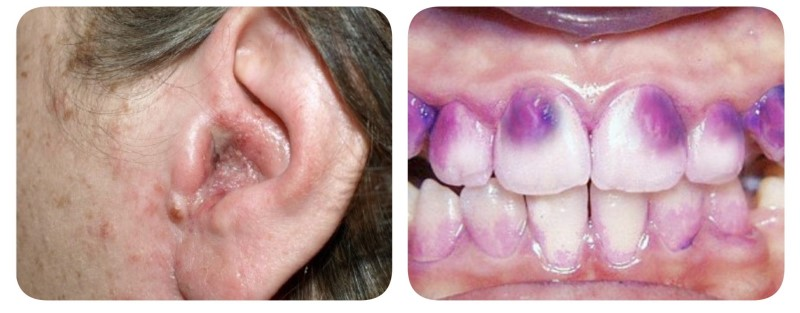
\includegraphics[width=0.45\linewidth]{chap-intro/output/biofilm-body}
}\qquad
\subfigure[In nature\protect\footnotemark.]{
  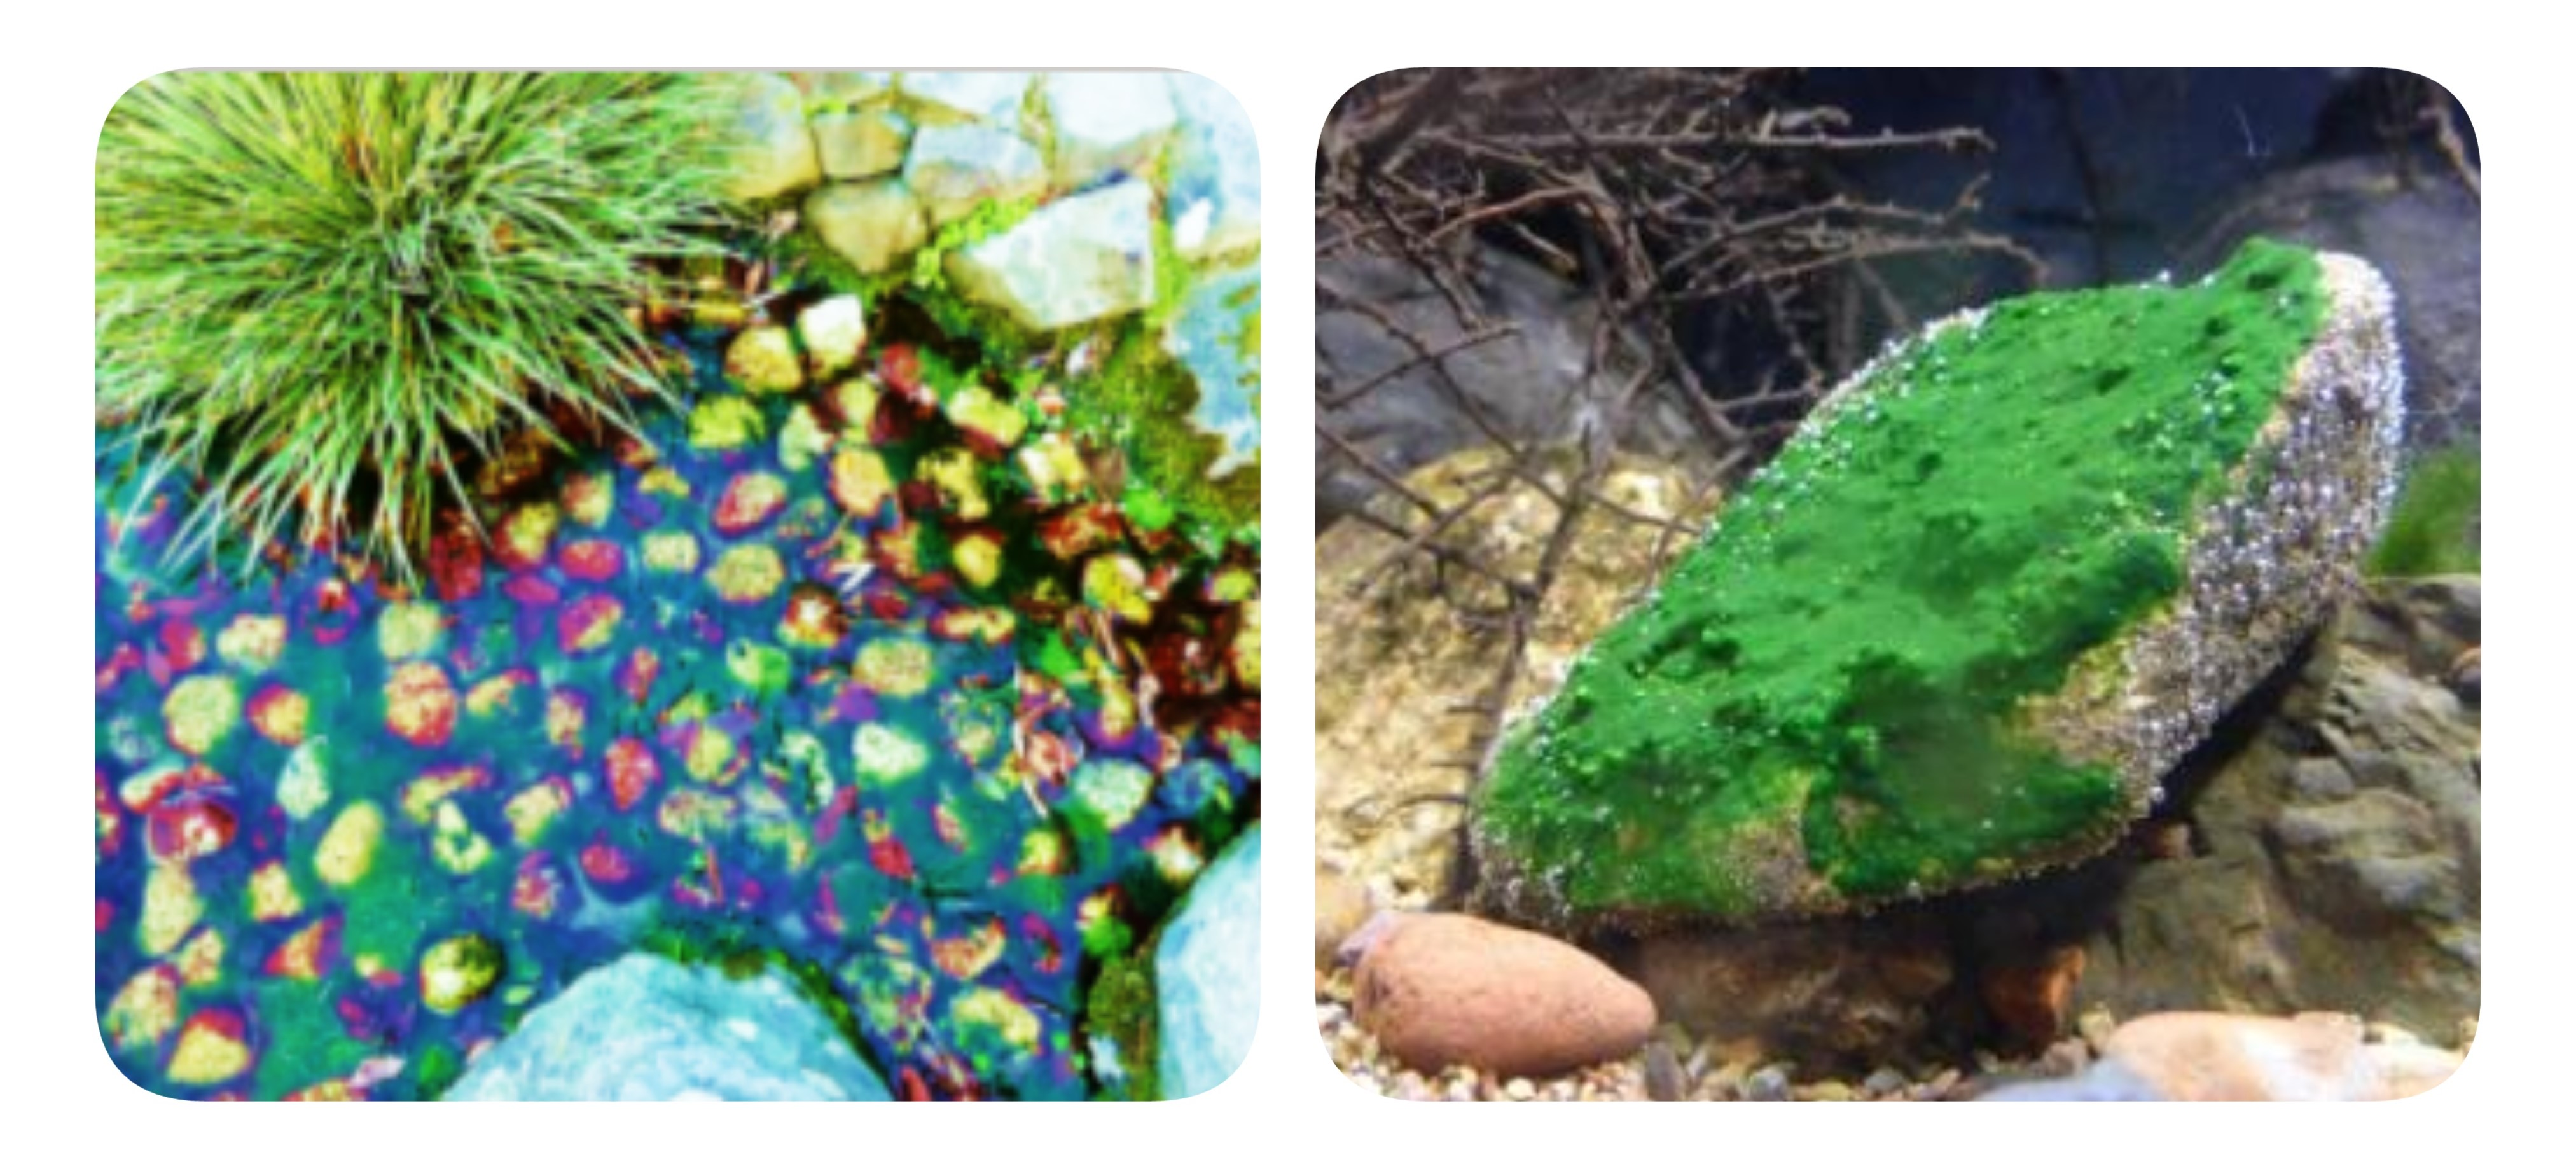
\includegraphics[width=0.43\linewidth]{chap-intro/output/bioflm-natural}  
}\\
\subfigure[In food\protect\footnotemark.]{
  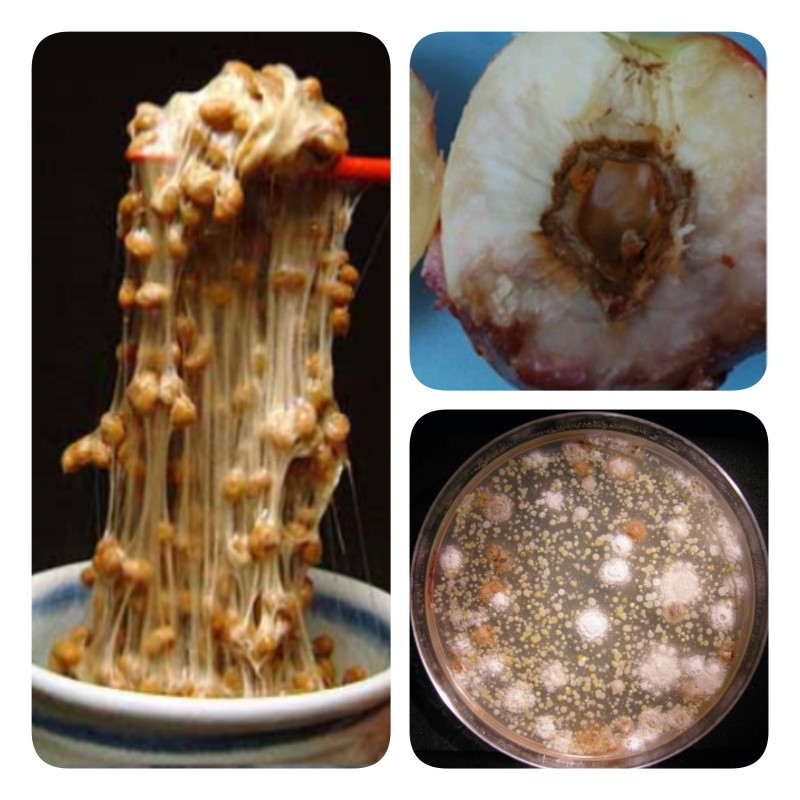
\includegraphics[width=0.41\linewidth]{chap-intro/output/biofilm-food}
}\qquad
\subfigure[Walter filter\protect\footnotemark.]{
  \label{subfig:biofilm-good}
  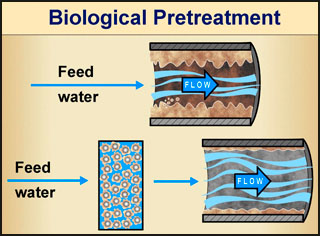
\includegraphics[width=0.49\linewidth]{chap-intro/output/biofilm-water-filter}
} %
\caption{Biofilm appears everywhere in human life.}
\label{fig:biofilm-in-life}
\end{figure}

\footnotetext[1]{Credit: Modification of work by Klaus D. Peter (ear) and bacteriality.com (teeth).}
\footnotetext[2]{Credit: skfaquatics.com.}
\footnotetext[3]{Credit: \textit{The strange case of a biofilm-forming strain of Pichia fermentans, which controls Monilinia brown rot on apple but is pathogenic on peach fruit} - Sara Giobbe \textit{et al}.}
\footnotetext[4]{Credit: P. Dirckx, Center for Biofilm Engineering, Montana State University, Bozeman.}

\begin{center}
  \begin{figure}[htp]
  \begin{center}
  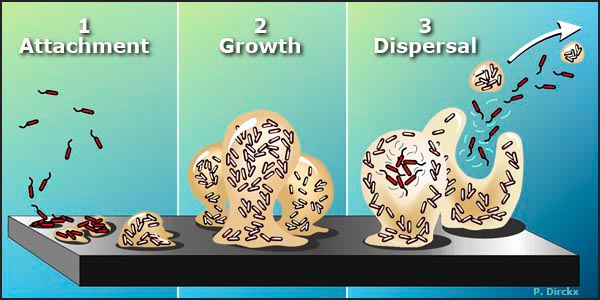
\includegraphics[width=\linewidth]{chap-intro/output/biofilm-life-circle}
  \end{center}
  \caption[Stages of the biofilm life cycle.]{Stages of the biofilm life cycle\protect\footnotemark.}
  \label{fig:biofilm-life-circle}
  \end{figure}
\end{center}

\footnotetext{Credit: Courtesy of the Montana State University Center for Biofilm Engineering, P. Dirckx.}

\begin{SCfigure}
  \centering
  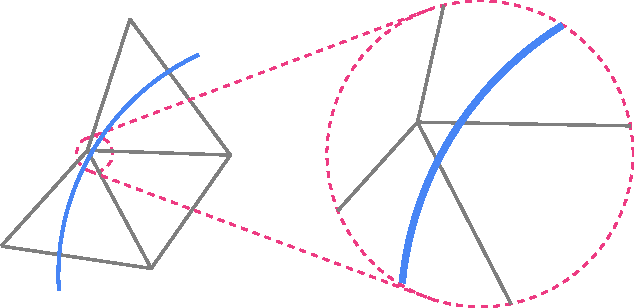
\includegraphics[scale=0.8]{chap-ori-nxfem/output/small-cut}
  \caption{Interface cuts triangle at positions which close to its vertex.}
  \label{fig:small-cut}
\end{SCfigure}

\begin{SCfigure}
  \centering
  \caption{An illustration of a fictitious domain $\Omg_{\mathcal{T}}$ of a physical domain $\Omega$.}
  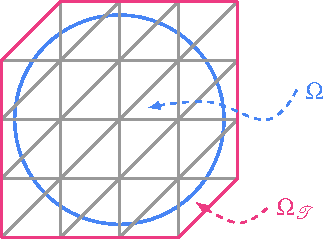
\includegraphics{chap-ori-nxfem/output/fictitious}
  \label{fig:fictitious-domain}
\end{SCfigure}


\section{Example of tables}

\begin{table}[ht]
  \centering
  {\tabulinesep=1.5mm
  % \taburowcolors[2] 2{white .. black!7}
  \setlength{\extrarowheight}{.75ex}
  \begin{tabu}{c | c | c | c | c}
    % \toprule
    \tableHeaderStyle
    $h$ & $\Norm{u_h-u_{\ex}}_{L^2}$ & order & $\vvvert{u_h-u_{\ex}}_H$ & order \\
		$9.52\times 10^{-2}$ & $7.3\times 10^{-3}$ &  & $0.51$ &  \\
    \tableRowStyle
    $4.88\times 10^{-2}$ & $1.7\times 10^{-3}$ & $1.82$ & $0.32$ & $0.7$ \\
		$2.47\times 10^{-2}$ & $3.91\times 10^{-4}$ & $2.01$ & $0.17$ & $0.9$ \\
    \tableRowStyle
    $1.24\times 10^{-2}$ & $9.97\times 10^{-5}$ & $1.93$ & $0.08$ & $1.1$
  \end{tabu}
  }
  \caption{$L^2, \Norm{\cdot}_H$ norm errors of the solutions with different mesh sizes in Barrau's test case.}
  \label{tab:chap2-error-barrau-x}
\end{table}

\begin{table}[ht]
  \centering
  {\tabulinesep=2mm
  % \taburowcolors[2] 2{white .. black!7}
  \setlength{\extrarowheight}{.75ex}
  % \begin{tabu}{c | c}
  \begin{tabu}to \linewidth{|X[c]|X[1.5,c]}
    % \toprule
    \tableHeaderStyle
    $\mbb{P}^1$-FE & $\mbb{P}^2$-FE \\
    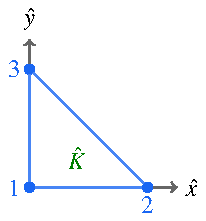
\includegraphics{chap-matlab/output/p1-tri} &
    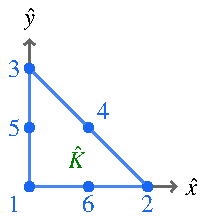
\includegraphics{chap-matlab/output/p2-tri}\\
    \tableRowStyle
    $\aligned
      N_1(\hx,\hy) &= 1-\hx - \hy, \\
      N_2(\hx,\hy) &= \hx, \\
      N_3(\hx,\hy) &= \hy.
    \endaligned$
    &
    $\aligned
      N_1(\hx,\hy) &= 1-3\hx - 3\hy + 2\hx^2 + 4\hx\hy + 2\hy^2, \\
      N_2(\hx,\hy) &= 2\hx^2-\hx, \\
      N_3(\hx,\hy) &= 2\hy^2-\hy, \\
      N_4(\hx,\hy) &= 4\hx\hy, \\
      N_5(\hx,\hy) &= 4\hy-4\hx\hy-4\hy^2, \\
      N_6(\hx,\hy) &= 4\hx-4\hx\hy-4\hx^2.
    \endaligned$\\
    function \code{getP1shapes} in the toolbox & function \code{getP2shapes} in the toolbox \\
    \lastLineStyle
  \end{tabu}
  }
  \caption[Local shape functions defined on reference triangle $\hat{K}$.]{Local shape functions defined on reference triangle $\hat{K}$ where $N_i(x_j)=\delta_{ij}$.}
  \label{tab:shape-functions}
\end{table}

\begin{table}[ht]
  \centering
  {\tabulinesep=2mm
  \setlength{\extrarowheight}{.75ex}
  \begin{tabu}to \linewidth{|X[c]|g|X[c]}
    % \toprule
    \tableHeaderStyle
    Type 0 & Type 2 & Type 4 \\
    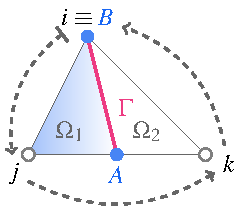
\includegraphics{chap-app-a/output/inter-type0-1} & 
    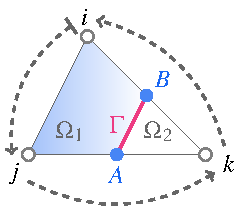
\includegraphics{chap-app-a/output/inter-type2-1} & 
    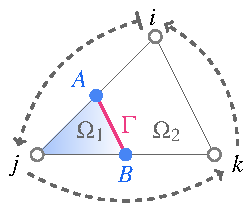
\includegraphics{chap-app-a/output/inter-type4-1} \\
    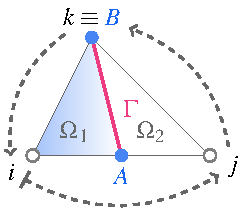
\includegraphics{chap-app-a/output/inter-type0-2} & 
    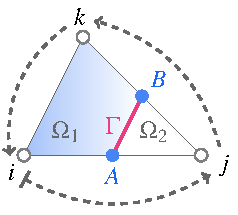
\includegraphics{chap-app-a/output/inter-type2-2} & 
    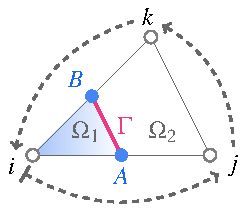
\includegraphics{chap-app-a/output/inter-type4-2} \\
    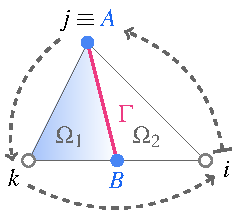
\includegraphics{chap-app-a/output/inter-type0-3} & 
    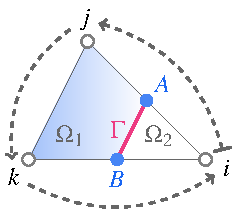
\includegraphics{chap-app-a/output/inter-type2-3} & 
    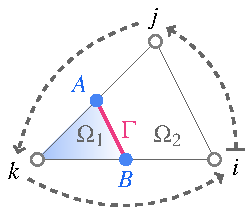
\includegraphics{chap-app-a/output/inter-type4-3} \\
    % \lastLineStyle
  \end{tabu}
  }
  \caption[Example of determining intersections between cut triangle and interface.]{Example of determining intersections between cut triangle \code{i-j-k} (in that order) and interface $\Gam_h$. They are all stored in \codeSM{CT.iPs} in order of $[A,B]$.}
  \label{tab:app-iPs}
\end{table}

\begin{table}[ht]
  \centering
  {\tabulinesep=2mm
  \setlength{\extrarowheight}{.75ex}
  \begin{tabu}to \linewidth{c|b|X[c]|X[c]|X[c]|X[c]|X[c]}
  % \begin{tabu}{b|c|c|c|c|c}
    \tableHeaderStyle
    figure & \multicolumn{6}{c}{cut triangles} \\
    \multirow{5}{*}{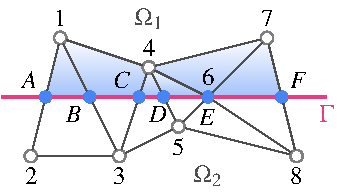
\includegraphics{chap-app-a/output/unv}} & i & $1$ & $3$ & $3$ & $6$ & $6$\\
    & j & $2$ & $4$ & $5$ & $4$ & $8$ \\
    & k & $3$ & $1$ & $4$ & $5$ & $7$ \\
    & \codeSMw{white}{CT.type} & $4$ & $2$ & $4$ & $0$ & $0$  \\
    & \codeSMw{white}{CT.iPs} & $[A,B]$ & $[C,B]$ & $[D,C]$ & $[D,E]$ & $[F,E]$  \\
    & $\text{\codeSMw{white}{CT.uN}}^{\perp}$ & $[B,A]$ & $[C,B]$ & $[D,C]$ & $[E,D]$ & $[F,E]$  \\
    % \lastLineStyle
  \end{tabu}
  }
  \caption[Example of determining unit normal vectors based on intersections]{Example of determining unit normal vectors \codeSM{CT.uN} based on intersections \codeSM{CT.iPs}. This result follows \algref*{alg:inter-points}. Note that, $\text{\codeSM{CT.uN}}^{\perp}$ is an orthogonal vector of \codeSM{CT.uN}.}
  \label{tab:app-unv}
\end{table}

\section{Example of mathematics expression}

\begin{align} \label{eq:ori-nxfem-bilinear-2}
  \begin{split}
    \abr{\nb u, \nb v}_{\Omg}
      & \underbrace{- \abr{\gradn u,v}_{\pt\Omg}}_{\color{tblue}\text{consistency}}
      - \underbrace{\abr{\gradn v,u}_{\pt\Omg}}_{\color{tgreen}\text{symmetry}}
      + \underbrace{\lam \abr{u,v}_{\pt\Omg}}_{\color{tpink}\text{stabilization}} \\
    &= \abr{f,v}_{\Omg}
      - \abr{g,\gradn v}_{\pt\Omg}
      + \lam \abr{ g,v }_{\pt\Omg}, 
      \quad \forall v\in H^1(\Omg).
  \end{split}
\end{align}

\begin{empheq}[box=\widefbox]{align}\label{eq:norm-tripleN}
  \vvvert{v}_N := \Norm{v}_{H^1(\Omg)}^2 + \sum_{E\in G_h} h_E^{-1} v^2\,dx,
\end{empheq}

\begin{align}\label{eq:ori-nxfem-hansbo}
  \begin{cases}
    -\nb\cdot (k\nb u) = f & \text{on } \Omg_1 \cup \Omg_2,\\
    \ssb{u} =0 & \text{on }\Gam, \\
    \ssb{k\gradn  u} = g & \text{on }\Gam, \\
    u = 0 &\text{on }\pt\Omg,
  \end{cases}
\end{align}

\section{Example of theorem styles}

\subsection{Assumption}

\begin{assumption}\label{ass:1}
We assume that $f\in L^2(\Omg), g\in H^{1/2}(\Gam)$ and $k$ is constant in $\Omg_i$ with $\alpha_i > 0$ for $i=1,2$.
\end{assumption}

\subsection{Remarks}

Som texts.

\begin{remark}[Cut triangle\index{cut triangle}]
  \label{rem:cut-triangle}
  A triangle is called a \textit{cut triangle} if the \assref*{ass:1} is satisfied and at least one cut point is not the vertex of this triangle. Some special cases of cut or not-cut triangles are given in \figref*{fig:small-cut}. Note that, we are considering a $\mathbb{P}^1$ - finite element space so $\Gam$ on each triangle is actually a line segment, that why we see all three cases a, b and c in \figref*{fig:small-cut} are the same. That is the reason why in the triangulation $\Th$, there is some triangle we see that it is cut by interface but it is still considered as a not-cut triangle (\figref*{fig:small-cut}).
\end{remark}

\subsection{Theorem, proposition and definition}

\begin{definition}
  \label{def:HOmg12}
  We use notation of function space $H^k(\Omg_{12})$ as follows,

  \begin{align*}
    H^k(\Omg_1\cup\Omg_2) 
      &= \{ v\in L^2(\Omg): v_i\in H^k(\Omg_i) \text{ for } i =1,2 \},
  \end{align*}
  
  for $k=0,1,2$ where $v_i=v\vert_{\Omg_i}$ and $H^0$ stands for $L^2$.
\end{definition}

\begin{theorem}\label{theo:interpolant-hansbo}\index{interpolant!estimate}
  Let $I_h^{\ast}$ be the interpolation operator defined in \eqref{eq:norm-tripleN}, then

  \begin{align*}
    \vvvert{u - I_h^{\ast}u}_H \le Ch\Norm{u}_{2,\Omg_{12}},
    \, \forall u \in H_0^1(\Omg) \cap H^2(\Omg_{12}).
  \end{align*}
\end{theorem}

\begin{proposition}\label{prop:jump-ave-prop}
  With the jump and average operators defined in \defref*{def:HOmg12} and $u,v$ two discontinuous functions across $\Gam$, we have,

  \begin{align*}
    \ssb{uv} &= \ssb{u}\bbrace{v} 
                + \bbrace{u}\ssb{v}
                + (\kap_2 - \kap_1)\ssb{u} \ssb{v} \text{ and }  \\
    \bbrace{uv} &= \bbrace{u}\bbrace{v}
                  + \kap_1\kap_2 \ssb{u}\ssb{v}.
  \end{align*}
\end{proposition}

\begin{proof}
  Denote $u_i=u\vert_{\Omg_i}, v_i=v\vert_{\Omg_i}$ for $i=1,2$, 

  \begin{align*}
    \ssb{uv} &= u_1v_1 - u_2v_2
      = \sum \kap_i u_1v_1 + \sum\kap_i u_2v_2 \\
      &= 2\kap_1 u_1v_1 - 2\kap_2 u_2v_2 
        + (\kap_2 - \kap_1)(u_1v_1 + u_2v_2) \\
      &= 2\kap_1 u_1v_1 - 2\kap_2 u_2v_2 
        + (\kap_2 - \kap_1)(u_1v_2 + u_2v_1)
        + (\kap_2 - \kap_1)\ssb{u}\ssb{v} \\
      &= \kap_1u_1v_1 + \kap_2u_1v_2 -\kap_1u_2v_1 -\kap_2u_2v_2 \\
        & \quad + \kap_1u_1v_1 - \kap_1u_1v_2 + \kap_2u_2v_1 - \kap_2u_2v_2 + (\kap_2 - \kap_1)\ssb{u}\ssb{v} \\
      &= \ssb{u}\bbrace{v} + \bbrace{u}\ssb{v} + (\kap_2 - \kap_1)\ssb{u}\ssb{v}.
  \end{align*}

  We also have

  \begin{align*}
    \bbrace{u}\bbrace{v} + \kap_1\kap_2 \ssb{u}\ssb{v}
      &= (\kap_1u_1 + \kap_2u_2)(\kap_1v_1 + \kap_2v_2)
        + \kap_1\kap_2(u_1-u_2)(v_1-v_2) \\
      &= \kap_1^2u_1v_1 + \kap_2^2u_2v_2 
        + \kap_1\kap_2 u_1v_1 + \kap_1\kap_2 u_2v_2 \\
      &= \bbrace{uv}.
  \end{align*}
\end{proof}

We can call \theoref*{theo:interpolant-hansbo} or \theoref*{theo:interpolant-hansbo}. For others, \propref*{prop:jump-ave-prop} and \defref*{def:HOmg12}.

\section{Example of bibliography}

There are 3 types of bibliography (articles \cite{Eymard2010,renard2009}, thesis \cite{Engwer2009,szomolayThesis} and books \cite{LeDret2013,Durr2009}). You even can do this \cite[Section~3]{George2000}.

\section{Example of Index}

You can use an index\index{index} or a group of indexes\index{main index!sub index}, \index{main index!sub index}

\section{Example of glossaries}

\glsadd{not:unv}, \glsadd{not:Th}, \glsadd{op:inner}, \glsadd{op:Interjump}, \glsadd{op:Interave}.




\end{document}